% chapter4 实验

\chapter{实验结果分析与模型评估}

\section{实验环境}

论文构建的HA-FuseNet是在实验室搭建的服务器上进行搭建和训练的,所用的软/硬件环境如表~\ref{tab:env}~所示:
\begin{table}[h]
    \centering
    \caption{实验环境}
    \label{tab:env}
    \begin{tabularx}{\textwidth}{>{\centering\arraybackslash\hsize=0.6\hsize}X >{\centering\arraybackslash\hsize=1.4\hsize}X}
    \toprule
    软/硬件名称 & 型号/版本 \\
    \midrule
    操作系统 & Ubuntu 20.04.6 LTS  \\
    CPU & Intel(R) Xeon(R) Gold 5218R CPU @ 2.10GHz \\
    GPU & NVIDIA GeForce RTX 3090 \\
    内存 & 128GB \\
    显存 & 24GB \\
    CUDA & 11.8 \\
    Python & 3.11.5 \\
    Pytorch & 2.0.1 \\
    MNE & 1.6.0 \\
    Numpy & 1.26.3 \\
    \bottomrule
    \end{tabularx}
\end{table}

\section{数据与实验准备}

\subsection{运动想象脑电图数据集}

运动想象脑电图是使用脑电采集设备从头皮上获取的人类大脑的神经元活动时产生的生物电电位信号,能够反映大脑皮层和深层结构的功能状态及其异常变化。脑电图信号的采集过程主要包括以下几个步骤:

(1) 采集准备:根据国际10-20标准导联系统或其他标准定位方案,将电极安放在被试头皮的不同位置,以捕获不同脑区的电位信号。电极通常通过电极帽或电极盘固定,以确保位置的稳定和正确。由于人体脑电信号强度微弱,通常会通过与脑电采集设备相连的放大器对脑电信号进行增强和记录;

(2) 信号记录:当大脑神经元兴奋或抑制时,会产生微弱的电位变化,这些电位变化传导到头皮表面,形成可测量的电压差,由脑电采集系统进行捕获和放大。脑电采集系统通常以每秒进行\(N\)次连续采集的方式工作,即采集频率为\(N\)Hz;

(3) 数字化:根据脑电采集系统的设置,对被捕获的脑电信号进行一定的处理,包括通过模数转换器(Analog to Digital Converter,ADC)将模拟信号转换为数字信号。

在临床和科研应用中,脑电图信号因其非侵入性、实时监测性、对大脑功能活动的敏感性等特点,已经在大脑解码领域获得了广泛的应用。运动想象领域有多个公开的脑电图信号数据集,论文主要选取BCI Competition IV Dataset 2A\cite{brunner2008bci}数据集和BCI Competition IV Dataset 2B\cite{leeb2008bci}数据集作为模型训练和测试的数据集。BCI Competition(脑机接口竞赛)是一项由德国柏林洪堡大学和柏林工业大学发起的国际性脑机接口技术竞赛,旨在推动脑机接口技术的创新和发展。在第四届比赛(BCI Competition IV)中,主办方提供了多项数据集,其中,运动想象领域的2A和2B数据集在相关研究中被广泛使用。

\paragraph{BCI Competition IV Dataset 2A}

BCI Competition IV Dataset 2A数据集采集了9名被试的MI-EEG信号,包括4类运动想象任务,即左手、右手、双脚和舌头。每名被试在不同的日期进行了两次采集/会话(session),两个session分别被作为训练集(T)和测试集(E),数据以.gdf的格式存储,因此,每名被试具有两个文件,如对于一号被试而言,存在A01T.gdf和A01E.gdf两个文件,其中,训练集A01T.gdf包含标签信息,A01E.gdf不包含标签信息,使用额外的A01E.mat文件提供标签。

session采集的过程如图~\ref{fig:2asession}~所示,在采集开始时,进行约五分钟的EOG记录,包括两分钟的睁眼模式、一分钟的闭眼模式和一分钟的眼球运动模式。其中,四号被试的测试集只具有眼球运动的EOG记录。
\begin{figure}
    \centering
    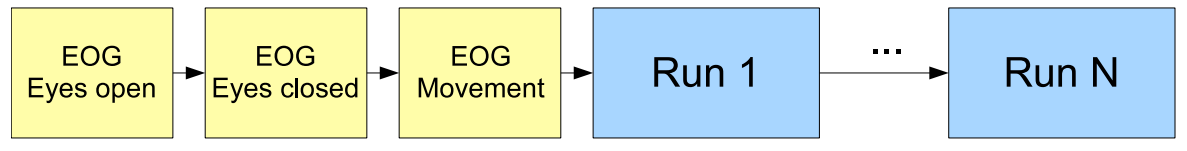
\includegraphics[width=0.8\textwidth]{2asession.png}
    \caption{2A session采集模式\cite{brunner2008bci}}
    \label{fig:2asession}
\end{figure}

在EOG记录之后,进行六次采集(run),在每个run中,各进行12次每类运动想象任务,这些任务的顺序是随机的,由此,一个run包含48次试验(trial),一个session包含288次试验(trial)。一个trial的流程如图~\ref{fig:2atrial}~所示,测试开始时(t=0s),一个十字图形出现在屏幕上,伴有简短的提示音;两秒后(t=2s),运动想象任务的指示箭头(分别指向左、右、下、上,对应左手、右手、双脚及舌头运动)出现在屏幕上,持续约1.25秒,每名被试进行运动想象任务直到十字图形消失(t=6s)。在这个过程中没有任何反馈。
\begin{figure}
    \centering
    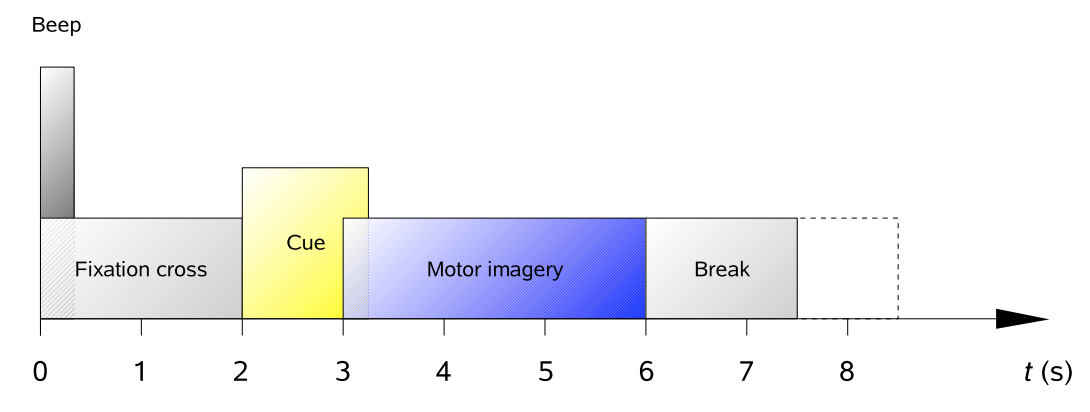
\includegraphics[width=0.8\textwidth]{2atrial.png}
    \caption{2A trial与无视觉反馈的2B trial的采集模式\cite{brunner2008bci,leeb2008bci}}
    \label{fig:2atrial}
\end{figure}

采集过程中,以250Hz进行EEG信号采样,并在0.5Hz至100Hz之间进行了带通滤波,放大器的灵敏度被设置为100\(\mu\)V,并使用了50Hz的陷波滤波器用以抑制线路噪声。头皮电极的位置按照国际10-20标准导联确定,共使用22个电极(通道),此外,还使用了3个不参与分类的EOG电极用以记录眼电信号。

在BCI领域,事件描述某一种波形或任务的起始点,数据上,事件表现为一个三元组:第一个元素以整数来描述的事件起始采样点;第二个元素对应当前事件来源的刺激通道(Stimulus Channel)的先前值(Previous Value),大多数情况下为0;第三个元素表示该事件的类型(Identify,id)。BCI Competition IV Dataset 2A数据集中共包含11类事件(Event),其中,与数据处理相关的事件如表~\ref{tab:2aevent}~所示,其中,拒绝试验是指由于质量欠佳或受试者未能有效完成而被专家标注出的试验数据。
\begin{table}[h]
    \centering
    \caption{2A事件类型列表}
    \label{tab:2aevent}
    \begin{tabularx}{\textwidth}{CC}
    \toprule
    事件类型 & 描述 \\
    \midrule
    768 & trial开始  \\
    769 & 左手运动想象任务(class 1) \\
    770 & 右手运动想象任务(class 2) \\
    771 & 双脚运动想象任务(class 3) \\
    772 & 舌头运动想象任务(class 4) \\
    783 & 未知运动想象任务(测试集) \\
    1023 & 拒绝试验 \\
    \bottomrule
    \end{tabularx}
\end{table}

论文遵循BCI Competition竞赛设置,使用T文件为训练集,E文件为测试集,针对每名被试进行被试内实验和被试间实验。则在不剔除拒绝试验数据的情况下,每名被试的训练集和测试集切片数量分别为:288,288。

\paragraph{BCI Competition IV Dataset 2B}

BCI Competition IV Dataset 2B采取了类似2A数据集的采集方式,采集了9名被试的2类MI-EEG信号(左手、右手),每名被试在不同时间进行了五次session,数据以.gdf格式存储,每名被试有五个文件,例如,对于一号被试而言,B0101T.gdf、B0102T.gdf和B0103T.gdf为训练集,、B0104E.gdf和B0105E.gdf为测试集。其中,前两个文件不包含视觉反馈,后三个文件包含视觉反馈,即在试验过程中,通过屏幕上的笑脸图案对运动想象任务是否被正确执行予以反馈。无视觉反馈的session包含6次run,每个run包含20次trial(左手、右手各10次,随机排布),有视觉反馈的session包含4次run,每个run包含40次trial(左手、右手各20次,随机排布)。无视觉反馈的trial的采集模式与2A相同,如图~\ref{fig:2atrial}~所示。

BCI Competition IV Dataset 2B的事件类型与2A的事件类型相似,但不包含双脚和舌头运动想象任务。此外,不同于2A数据集的22个电极,2B数据集仅使用3个电极记录数据。

为了保证实验数据只涉及运动想象,而不涉及视觉反馈,论文选择无视觉反馈的两个session分别作为训练集和测试集,则在不剔除拒绝试验数据的情况下,每名被试的训练集和测试集切片数量分别为:120,120。

综上所述,论文所使用的数据的信息如表~\ref{tab:dataset}~所示。
\begin{table}[ht]
    \centering
    \caption{数据集信息}
    \label{tab:dataset}
    \begin{tabularx}{\textwidth}{CCC}
      \toprule
      数据集 & BCI IV 2A & BCI IV 2B \\
      \midrule
      被试数量 & 9 & 9 \\
      类别数量 & 4 & 2 \\
      通道数量 & 22 & 3 \\
      频率范围 & 0.5-100Hz & 0.5-100Hz \\
      采样频率 & 250Hz & 250Hz \\
      训练集数据量 & 288(每被试) & 120(每被试) \\
      测试集数据量 & 288(每被试) & 120(每被试) \\
      \bottomrule
    \end{tabularx}
\end{table}

\subsection{数据预处理}

EEG信号具有低信噪比、非平稳、空间变异性等特性,并且通常具有较小规模的数据集,一般来说,对数据进行一定的预处理有助于后续分类任务。然而,论文基于端到端网络的思想构建模型,因此尽可能地对预处理操作进行削减。论文进行的数据预处理方法如下:

\paragraph{数据提取与切片}

MI-EEG原始信号储存在.gdf格式的文件中,除目标脑电信号之外,原始文件还包括EOG信号、间隙缺失值、与运动想象任务不直接相关的事件等。因此,在提取数据时,有必要进行一定的处理:

首先,剔除EOG通道数据,仅保留EEG通道数据,对于用于分隔run的缺失值(编码为非数字,NaN),使用对应通道的均值替代,以确保数据的连续性和完整性;

其次,对与运动想象任务直接相关的事件进行筛选和提取,并对相关时段进行切分。对于BCI Competition IV的2A/2B数据集,直接相关事件为四类/二类运动想象任务事件,并由提示信号(Cue)标识任务的开始,论文对连续数据进行切片,提取从Cue出现后的第1秒至第4秒(trial周期的第3秒至第6秒)的数据段,作为事件对应的运动想象任务持续期间产生的EEG信号,在后续加以分析。对于采样率为250Hz的数据集而言,3秒的数据区间将包含750个采样点。

需要说明的是,论文在数据提取过程中并未对拒绝试验进行剔除,同时未使用滤波器对EEG信号的频率进行过滤,以对真实应用情境中可能出现的多样化数据表现进行模拟,对模型自主识别各种频率成分并提取有效特征的能力进行评估。

\paragraph{标准化}

归一化操作的目的在于对数据的特征尺度进行统一,从而消除奇异数据导致的不良影响,提高模型的训练效率和稳定性。EEG信号常用的归一化方法有Z-score标准化、最大最小值归一化等。

Z-score标准化的操作过程如公式~\ref{eq:z-score}~所示,其中,x为原始数据,\(\mu\)表示数据的均值,\(\sigma\)表示数据的标准差,Z-score通过均值和标准差对数据进行操作,使得处理后的数据符合均值为0,方差为1的标准正态分布。
\begin{equation}
    x=\frac{x-\mu}{\sigma}
    \label{eq:z-score}
\end{equation}

最大最小值归一化的操作过程如公式~\ref{eq:maxmin}~所示,其是一种线性变换操作,将数据映射至\([0,\,1]\)区间,其中,\(X\)为一组通道数据。最大最小值归一化计算简单,但对具有波动性的EEG信号而言,将数据缩放至\([0,\,1]\)区间容易导致数据特征的损失。
\begin{equation}
    x=\frac{x-min(X)}{max(X)-min(X)}
    \label{eq:maxmin}
\end{equation}

因此,为了尽可能保留EEG信号的特征,论文采用Z-Score标准化方法对EEG信号进行处理,以提高模型训练的速度和稳定性。

\paragraph{数据增强}

MI-EEG信号通常具有较小规模的数据集,因此,通过一定的数据增强操作扩大数据规模,有助于提升网络训练效果,防止过拟合现象的发生。然而,在BCI系统的实际应用中,数据增强操作可能会导致训练阶段数据处理压力的增长,因此,在论文中,数据增强是一项可选操作,其目的在于提高模型分类精度,论文将分别使用进行数据增强和不进行数据增强的数据集进行训练。

EEG信号的数据增强方法主要有以下几种:

(1) 添加随机噪声:在EEG信号上叠加高斯白噪声、有色噪声等不同类型的噪声,模拟真实环境中的噪声干扰,能够提升模型的抗噪性和鲁棒性;

(2) 滑动窗口:设定时间滑动窗口的长度小于运动想象任务持续的时间长度,将滑动窗口内的数据视作一次事件,通过滑动窗口对数据进行切片,有助于模型学习EEG信号随时间变化的特征;

(3) 频率混叠:在保持EEG信号特性的前提下,将多种不同频率成分进行混叠,使得模型能够学习更广泛的频率特征。

由于在预处理阶段没有采取频率滤波的操作,论文采取频率混叠的方式对EEG信号进行增强,从而加强模型识别不同频率成分的能力。具体算法流程如算法~\ref{alg:aug}~所示。
\begin{algorithm}[H]\label{alg:aug}
    \caption{数据增强算法}
    \SetAlgoLined
    \KwData{Dataset for every subject $X=\{x_1, x_2, ..., x_9\}$ and the $subject\_id$ to be augmented.}
    \KwResult{augmented dataset for every subject $Y=\{y_1, y_2, ..., y_9\}$.}
    $Y = []$ \;
    \For{each item $x_i \in X$}{
        $X' = $ selected $x_j$ from $X,\,j \neq i,\,j \in [1,2,...,9]$ \;
        $y_i = x_i$ \;        
        $x_i = $ crop $x_i$ from where the first trial begins\;
        $x_i = $ filter $ x_i $ into $ [4Hz,40Hz] $ \;
        \For{each item $s_i \in X'$}{
            $s_i = $ crop $s_i$ from where the first trial begins\;
            $s1_i = $ filter $ s_i $ into $ [0.5Hz,4Hz)$ \;
            $s2_i = $ filter $ s_i $ into $ (40Hz,100Hz)$ \;
            $y_i = $ concatenate $ (y_i, s1_i+x_i+s2_i)$ \;
        }
        $Y = Y$ append $y_i$ \;
    }
    \Return{$Y$}\;
\end{algorithm}

\subsection{实验准备}

\paragraph{评价指标}

论文主要使用准确率(Accuracy,Acc)、Kappa一致性系数(Kappa)和标准差(Standard Deviation,SD)作为模型的评价指标。其中,准确率是分类任务中常用的评价指标,用于衡量模型预测结果与真实标签相匹配的比例,其计算方式为正确分类的样本数占总样本数的比例。

Kappa一致性系数用于衡量模型预测结果与真实标签之间的一致性程度,在类别不平衡或随机猜测具有一定效果的情况下,Kappa一致性系数尤其有效。Kappa系数基于混淆矩阵进行计算,其计算公式如下:
\begin{equation}\label{eq:kappa}
    Kappa=\frac{P_o-P_e}{1-P_e}
\end{equation}
其中,\(P_o\)为观察一致性(Observed Proportion of Agreement),即准确率,\(P_e\)为预期一致性(Expected Proportion of Agreement by Chance),假设样本总量为\(N\),类别总量为\(c\),第\(i\)类的真实样本个数为\(x_i\),预测样本个数为\(p_i\),则\(P_e\)的计算公式如~\ref{eq:pe}~所示。
\begin{equation}\label{eq:pe}
    P_e=\frac{\sum_{i=1}^{c}t_i \times p_i }{N^{2} } 
\end{equation}
Kappa系数的范围在-1至1区间内,通常大于0,Kappa值越大,表明一致性程度越高,当Kappa值位于[0.61,0.80]区间时,表示预测与真实具有高度的一致性。

标准差用于衡量模型在不同被试之间的稳定性能力,其值越小,表明不同被试的准确率越相近,模型的稳定性越好。其计算公式如下:
\begin{equation}
    SD=\sqrt{\frac{1}{N-1}  \sum_{i=1}^{N}(x_i-\bar{x} )^{2} } 
    \label{eq:sd}
\end{equation}
其中,\(N\)表示被试数量,\(x_i\)表示第\(i\)个被试的准确率,\(\bar{x}\)为\(N\)个被试准确率的平均值。

\paragraph{损失函数及参数配置}

论文使用交叉熵损失函数(Cross Entropy Loss)。交叉熵的概念源自于信息论,用于衡量两个概率分布之间的差异性,交叉熵的值越小,表明两个概率分布越相似,因此,可以通过最小化交叉熵的方式,使得一个概率分布逼近目标概率分布。

交叉熵损失函数是一类在分类任务中广泛应用的损失函数,能够衡量模型预测值与真实标签之间的差异,其计算公式如下:
\begin{equation}
    L= -\sum_{i=1}^{C}y_i log(\hat{y}_i )
    \label{eq:loss}
\end{equation}
其中,\(C\)为分类类别数,\(y_i\)表示真实类别,\(\hat{y}_i\)表示模型预测的类别\(i\)的概率。交叉熵损失函数使用真实标签对模型预测的结果进行惩罚,从而促使模型学习到更为准确的预测结果。

论文使用Adam优化算法。对于2A数据集,批大小(batch size)设置为32,2B数据集设置为20;实验迭代次数(epochs)设置为300次;初始学习率(learning rate)设置为1e-3,权重衰减值(weight decay)设置为5e-3。

\section{实验设计}

\subsection{DIS-Net实验设计}

为了确定模型架构的最佳设置,本节对DIS-Net构建过程中不同的模型架构进行实验,从而逐步构建起性能最优的模型。

\paragraph{Inception模块引入空间卷积层的方式}

在DI-Net中,空间卷积层有两种不同的方式融入基于Inception改进的时间卷积层之后,一种是在每个Inception模块内部的分支结构上增加空间卷积层,另一种则是在整个Inception模块之后附加空间卷积层。图~\ref{fig:ts-incep}~展示了这两种引入方式的区别,将这两种方式分别称为分支内融合(Inception-In)和模块后融合(Inception-After),需要说明的是,图中省略了网络的其他结构,如瓶颈层等,以尽可能简洁地展现不同引入方式的差异。其中,\(s\_kernel\)表示空间卷积核,\(t\_kernel_i\)表示第\(i\)个分支的时间卷积核。
\begin{figure}
  \centering
  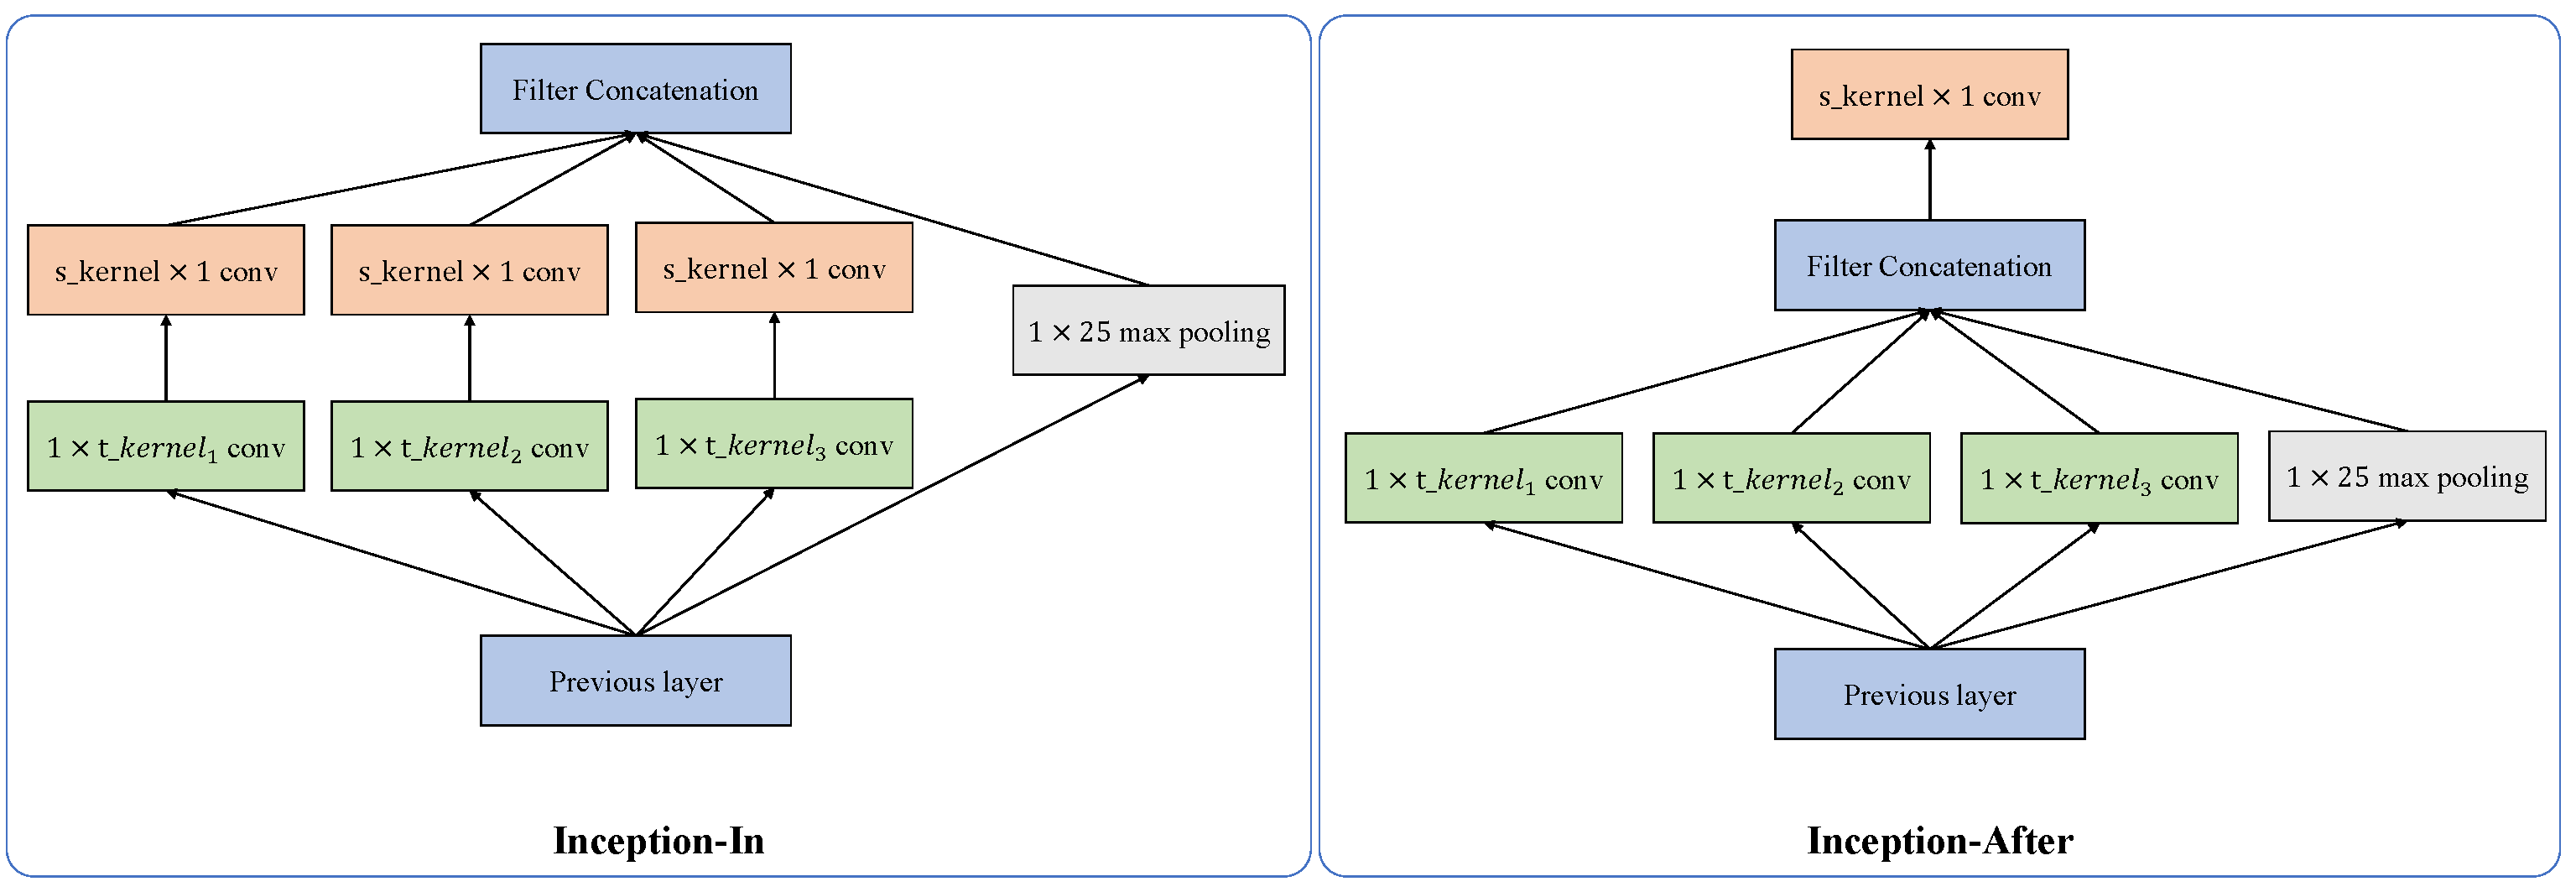
\includegraphics[width=\textwidth]{ts-incepv3.pdf}
  \caption{Inception模块引入空间卷积层的方式}
  \label{fig:ts-incep}
\end{figure}

为了比较Inception-In与Inception-After的性能差异,论文在BCI Competition IV Dataset 2A数据集上设计实验进行对比。在实验设置阶段,固定了Inception模块的层次数量、分支数量等参数,实验结果如表~\ref{tab:ts-inception}~所示。表格中的两项指标均基于数据集中九位被试的平均表现。实验结果显示,Inception-After方式在准确率和一致性系数上均表现更优。这一优势可能源自两方面的原因:一方面,虽然Inception-In模式借鉴了FBCSP算法的分频段处理思路,但在Inception分支内部直接进行空间特征提取的过程中,损失了部分空间全局信息;另一方面,Inception-In结构具有相对更大的参数规模,这可能导致模型在有限样本条件下更容易出现过拟合现象。基于以上分析和实验验证,论文选择以Inception-After的方式布局时间卷积层与空间卷积层。
\begin{table}[ht]
  \centering
  \caption{Inception-In、Inception-After实验结果对比}
  \label{tab:ts-inception}
  \begin{tabularx}{\textwidth}{CCC}
    \toprule
    Models & ACC(\%) & Kappa \\
    \midrule
    Inception-In & 63.31 & 0.51 \\
    Inception-After & \textbf{75.35} & \textbf{0.70} \\
    \bottomrule
  \end{tabularx}
\end{table}

\paragraph{svSE模块引入的对比试验}

为了选择适合MI-EEG分类任务的基准注意力机制,论文在DI-Net的时间卷积层后引入了不同的混合注意力模块,并在2A数据集上进行了实验,实验结果如表~\ref{tab:att}~所示,表中的指标为九位被试的平均表现,由于scSE模块取得了最好的表现,论文选择基于scSE模块进行改进。
\begin{table}[ht]
    \centering
    \caption{不同注意力模块引入DI-Net的实验结果对比}
    \label{tab:att}
    \begin{tabularx}{\textwidth}{CCC}
      \toprule
      Attention & ACC(\%) & Kappa \\
      \midrule
      CBAM\cite{woo2018cbam} & 74.97 & 0.64 \\
      scSE\cite{8578843} & 76.35 & 0.69 \\
      CoordAttention\cite{Hou2021CoordinateAF} & 71.84 & 0.62 \\
      \midrule
      svSE & 78.09 & 0.71 \\
      \bottomrule
    \end{tabularx}
\end{table}
在表~\ref{tab:att}~中,同样展示了svSE以同样方式引入DI-Net的效果,以展示其改进的有效性。svSE在四类混合注意力机制中取得了最高的准确率和Kappa系数。

DIS-Net中,由于DI-Net的特征提取过程分为时间卷积和空间卷积两个阶段,svSE模块可采取以下三种引入方式:其一是在时间卷积层后引入;其二是在空间卷积层后引入;其三是同时在时间卷积层和空间卷积层之后引入。图~\ref{fig:att-Base}~展示了这三种引入svSE模块的方式,从左至右分别是时间卷积层后引入svSE模块、空间卷积层后引入svSE模块,以及在时间卷积和空间卷积层后均引入svSE模块。将这三种引入方式对应的模型分别简称为S-Temporal-Net、S-Spatial-Net、S-TS-Net。
\begin{figure}
  \centering
  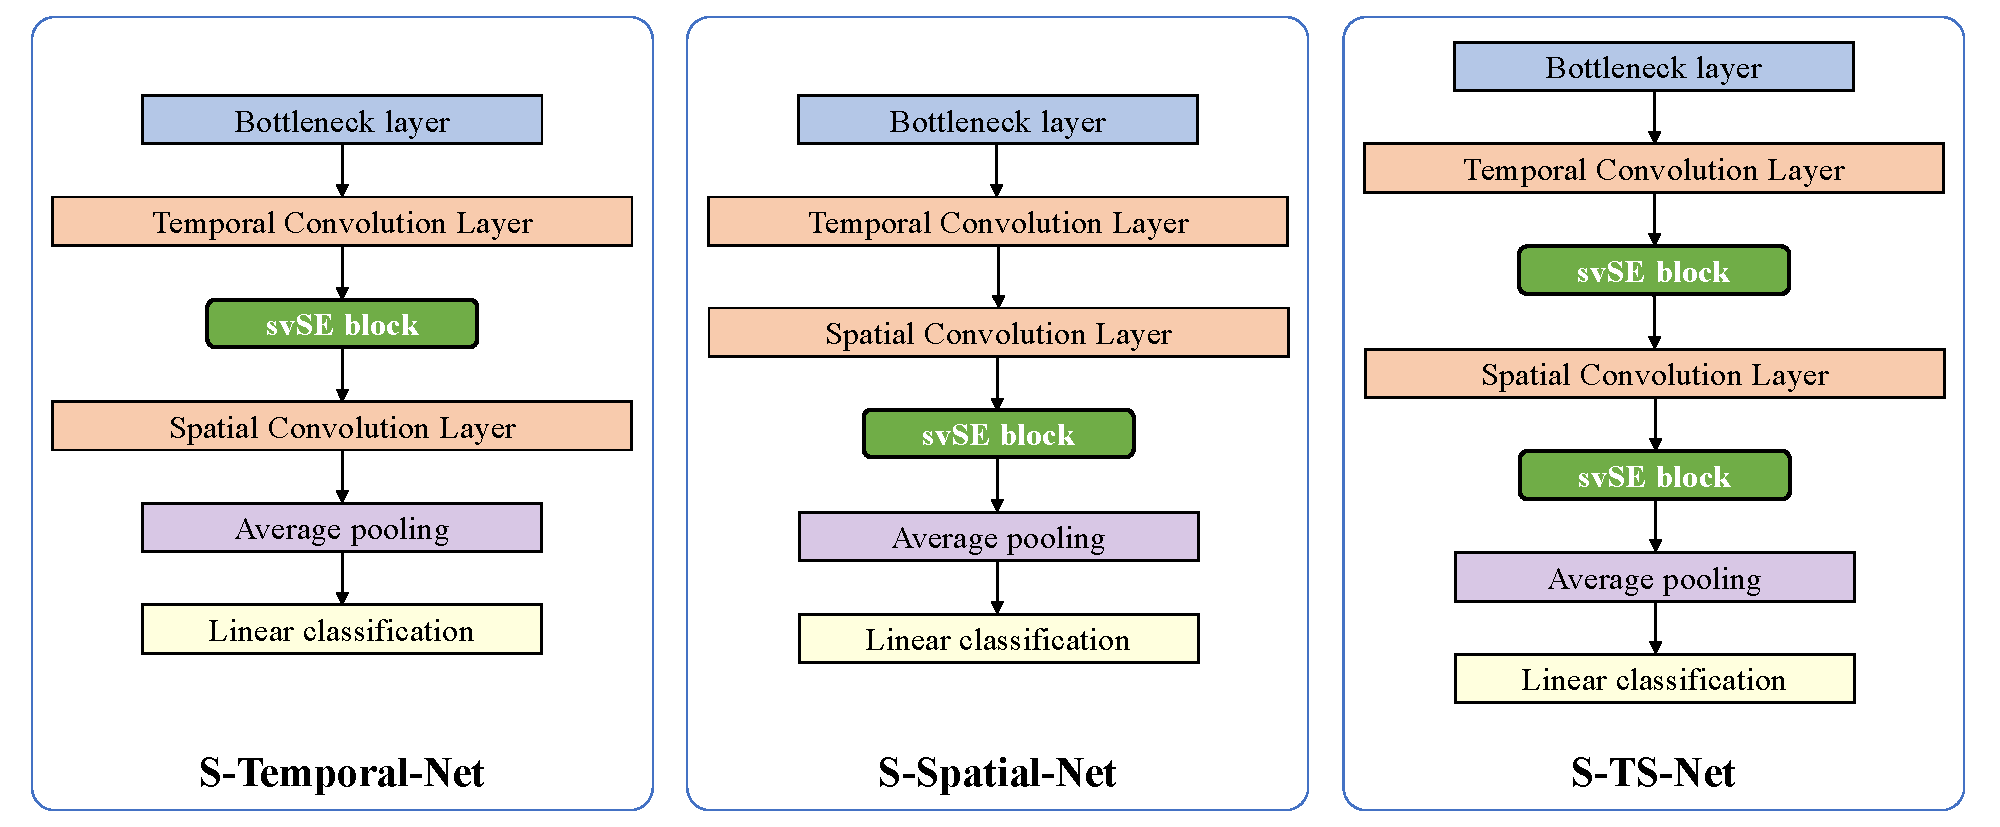
\includegraphics[width=\textwidth]{att-Basev2.pdf}
  \caption{DI-Net引入注意力模块的方式}
  \label{fig:att-Base}
\end{figure}

表~\ref{tab:svSE-BaseNet}~展示了S-Temporal-Net、S-Spatial-Net、S-TS-Net三种模型在2A数据集上的对比实验结果。表格中的指标为数据集中九位被试的平均表现。从准确率和一致性分析,S-ST-Net模型的效果优于其他两种模型,与经验相符。此外,S-Temporal-Net模型的效果优于S-Spatial-Net模型,其原因可能在于,空间卷积层沿通道维度的卷积使得数据损失了部分特征,进而减弱了svSE模块提取关键特征权重的能力,而时间卷积层保留了大部分深度信息和通道信息,因此,在时间卷积层之后加入svSE模块能够帮助模型更好地捕捉深度和空间的特征。从标准差分析,S-TS-Net模型的准确率波动幅度较小,对不同被试的MI-EEG分类效果相对均衡,另外两种模型在不同被试间的分类精度则存在较为明显的差异。实验数据显示,S-TS-Net模型取得了更好的效果,因此,论文采用同时在时间卷积层和空间卷积层之后引入svSE模块的方式,将这种结构的模型称为DIS-Net。
\begin{table}[ht]
    \centering
    \caption{svSE模块引入位置对比}
    \label{tab:svSE-BaseNet}
    \begin{tabularx}{\textwidth}{CCCC}
        \toprule
        Models & ACC(\%) & Kappa & SD \\
        \midrule
        S-Temporal-Net & 78.09 & 0.71 & 10.38 \\
        S-Spatial-Net & 77.16 & 0.69 & 10.24 \\
        S-TS-Net & \textbf{78.55} & \textbf{0.71} & \textbf{9.46} \\
        \bottomrule
    \end{tabularx}
\end{table}

\paragraph{不同轻量化模块对比}

为了对模型进行轻量化,论文在SG模块之外,基于ShuffleNetV2提出了GAS/SAS模块。
ShuffleNetV2问题在于,进行Channel Split时,通常是对特征图进行均匀划分,难以灵活调整直传特征图的比例,可能导致对重要特征信息的有效利用率不足。此外,ShuffleNetV2的基础结构在深度维度上的特征变换主要依赖于\(1\times1\)卷积,这在一定程度上限制了其内在的深度特征变换能力。

为了提升ShuffleNetV2基本模块在深度特征变换方面的能力,论文提出了一种可调节分支比例的Shuffle模块(Adaptive Shuffle Module, AS模块),其架构如图~\ref{fig:as}~(a)所示。假设卷积层的输入深度为 \(D_{in}\),输出深度为 \(D_{out}\),针对不同的输入输出深度关系(即 \(D_{in} \le D_{out}\) 和 \(D_{in} > D_{out}\) ),论文对AS模块进行了优化,分别形成了图~\ref{fig:as}~(b)所示的GAS模块(Growing Adjustable Shuffle Module)和图~\ref{fig:as}~(c)所示的SAS模块(Straight Adjustable Shuffle Module)。图中的DW Conv指深度卷积(Depthwise Convolution),\(ratio\)为可调的权重参数。
\begin{figure}
    \centering
    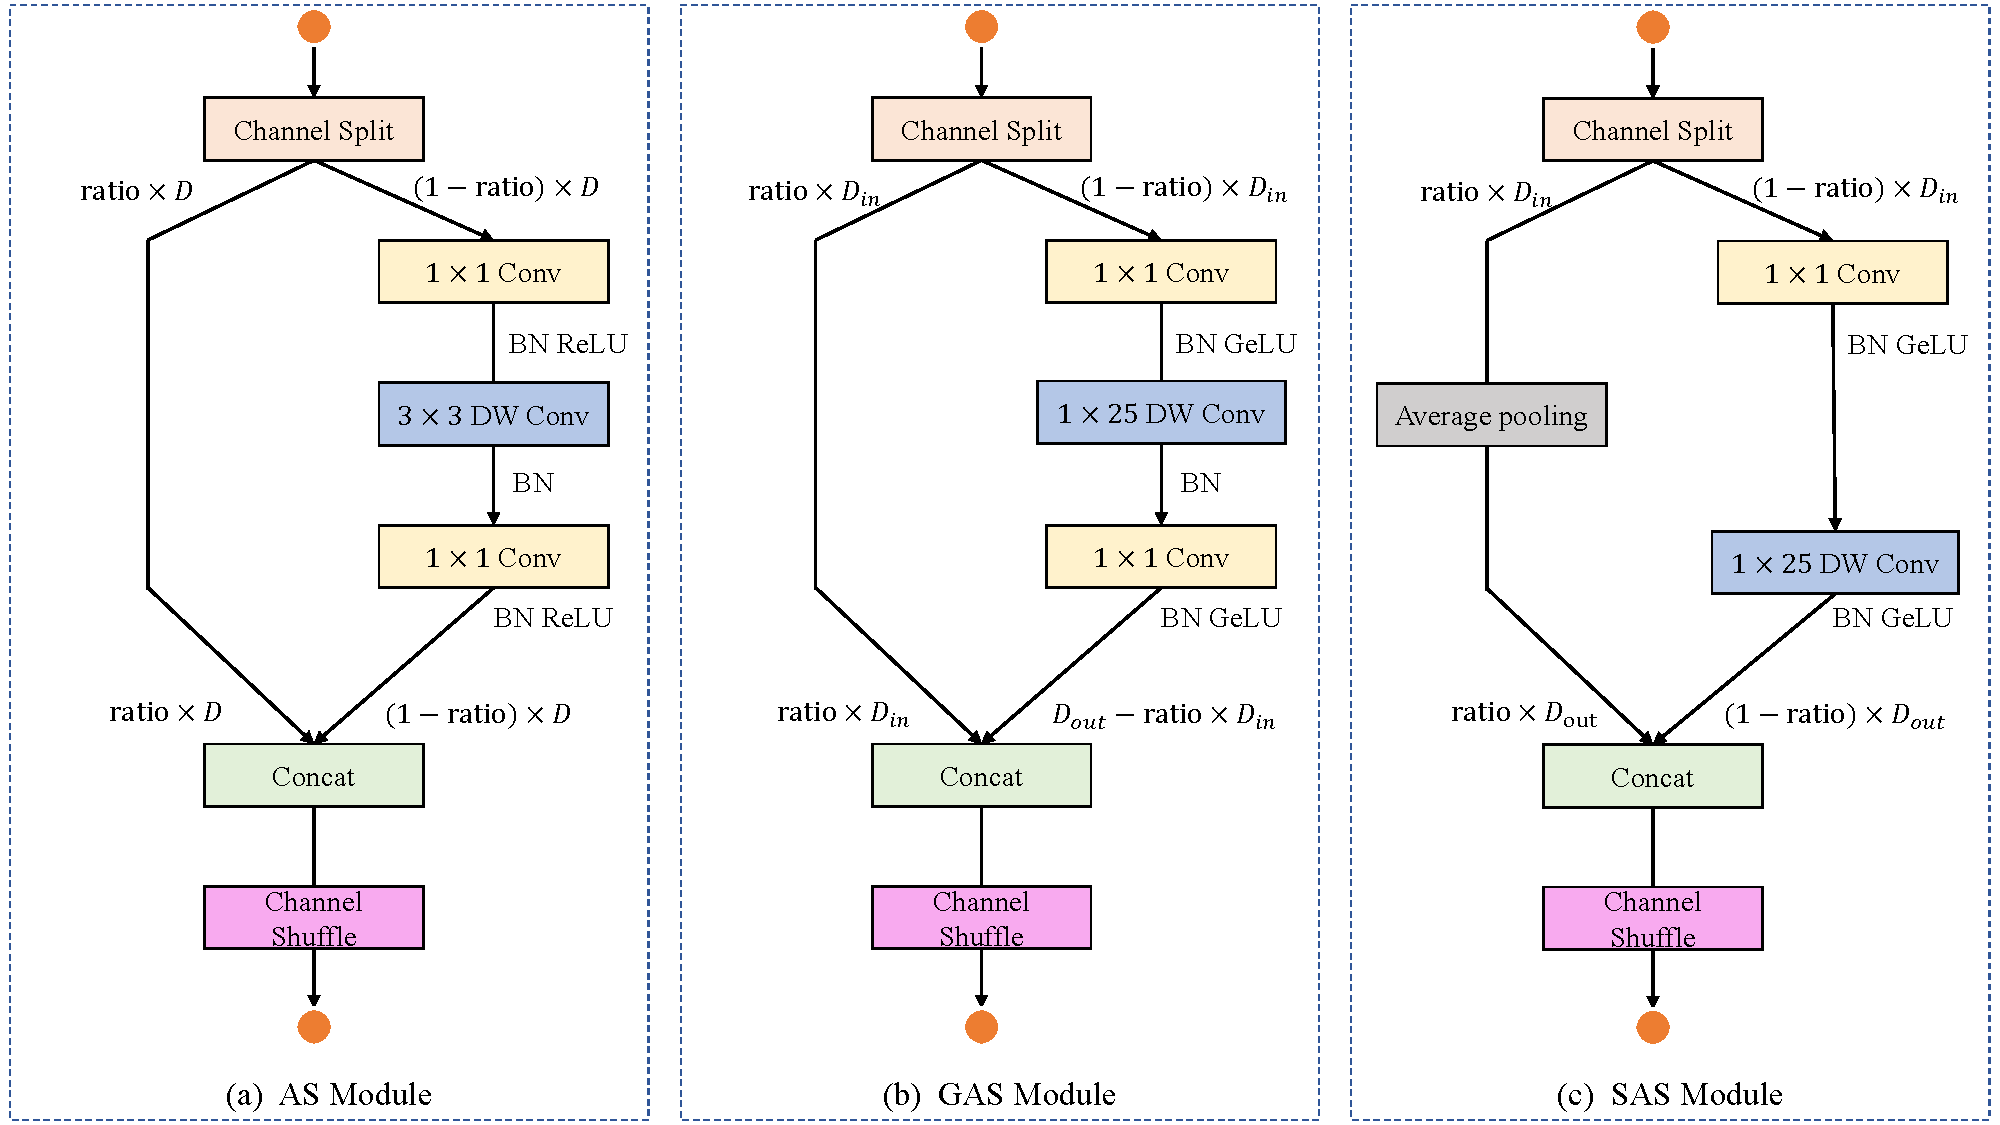
\includegraphics[width=\textwidth]{AS.pdf}
    \caption{AS、GAS、SAS模块结构}
    \label{fig:as}
\end{figure}

对于GAS模块,在保留原有直接传递分支的同时,改动了深度变换的分支的卷积核大小和激活函数,以优化GAS模块对MI-EEG分类任务的性能。对于SAS模块,其在变换分支的设计上采用了与GAS模块一致的改进措施,但去掉了最后的\(1\times1\)卷积层,而由第一个\(1\times1\)卷积层将深度降维至输出维度,再由\(1\times25\)卷积层进行特征的提取。此外,在直接传递分支上,进一步引入了深度维度上的平均池化操作,目的在于在不增添额外参数的前提下,有效减少特征图的数量。相较于原始的Shuffle unit,GAS模块和SAS模块在功能上进行了扩展,不仅包含了特征维度的升维和降维处理,而且还引入了一个可调节的权重参数 \(ratio\),以动态控制两个分支的特征图数量,从而在处理MI-EEG分类任务时,能够更加灵活和高效地调整特征空间的分布和深度特征的提取。

论文针对通道混洗算法进行了优化升级,使其具备了对不同数量分组及不同数量组内特征图进行灵活、均衡混洗的能力。这使得无论待重排的组及组内特征图的数量如何变化,该算法都能够实现有效的特征交互与信息整合。

为了验证更适合的轻量化卷积模块,论文在BCI Competition IV Dataset 2A数据集上进行了实验验证。由于轻量化卷积主要针对密集连接进行改进,实验使用DI-Net,并固定了Inception层数、密集连接层数、\(ratio\)等超参数。表~\ref{tab:lite}~展示了GAS/SAS、SG、Ghost和原始密集连接(Origin)模块的对比实验结果,其指标为参数量(Parameters)、浮点运算数(Floating Point Operations,FLOPs)和准确率,其中,准确率为九位被试的平均值。
\begin{table}[ht]
    \centering
    \caption{轻量化卷积模块实验结果对比}
    \label{tab:lite}
    \begin{tabularx}{\textwidth}{CCCC}
      \toprule
      Models & Paramters & FLOPs & ACC(\%) \\
      \midrule
      GAS/SAS & 7.31K & 130.37M & 74.61\\
      SG & 7.36K & 133.04M & \textbf{76.54}\\
      Ghost & \textbf{7.27K} & \textbf{129.93M} & 73.03\\
      \midrule
      Origin & 29.99K & 690.37M & 75.62\\
      \bottomrule
    \end{tabularx}
\end{table}
数据显示,Ghost模块具有最优的轻量化效果,而SG模块取得了最优的性能,甚至超出了原始密集连接模块。这可能是增加卷积层的深度有利于对特征的拟合,而较小的参数规模降低了过拟合的风险。此外,MobileNet证实在CPU上,计算量不变的情况下增加网络的层数有助于命中缓存,从而增加CPU上的计算速度。

实验证明,相较于原始密集连接模块,SG模块的轻量化效果明显;相较于Ghost模块、GAS/SAS模块和原始密集连接模块,SG模块取得了更优的性能。这证明了SG模块的有效性。

\subsection{LS-Net实验设计}

LS-Net中,SCoT模块引入LSTM的方式,以及LS-Net与DIS-Net进行特征融合的方式并不固定,因此,论文通过实验选择最优的架构。

\paragraph{SCoT引入LSTM的方式}

SCoT引入LSTM的方式有两种:在LSTM Layer之前,称之为SCoT-before;在LSTM Layer之后,称之为SCoT-After。为了比较两种方式的优劣,论文在2A数据集上使用HA-FuseNet进行实验,在实验中,固定了相关的超参数。
\begin{table}[ht]
    \centering
    \caption{SCoT引入LSTM实验结果对比}
    \label{tab:ls}
    \begin{tabularx}{\textwidth}{CCCC}
      \toprule
      Models & ACC(\%) & Kappa & SD \\
      \midrule
      SCoT-Before & 74.25 & 0.65 & 12.49 \\
      SCoT-After & \textbf{75.66} & \textbf{0.67} & \textbf{9.71} \\
      \bottomrule
    \end{tabularx}
\end{table}

实验数据显示,SCoT-After具有更高的准确率、一致性,以及更低的标准差,这证实了在LSTM Layer之后引入SCoT的方式具有更好的性能。这可能是因为,相较于前加权,后加权的方式直接对经过特征提取的特征图进行加权,加权后的特征图不再继续通过网络,从而更好地突出重要特征,促使模型学习到数据中更为重要的部分。

\paragraph{特征融合的方式}

LS-Net与DIS-Net以并行结构级联主要是出于以下考虑:

(1) CNN可以并行计算,LSTM由于按时间序列依次对数据进行计算,使得自身无法并行计算,因此在计算效率上低于CNN。如果使用串联方式,会导致LS-Net与DIS-Net无法并行计算,降低HA-FuseNet的计算效率。需要说明的是,论文通过下采样的方式提高LS-Net的计算效率。

(2) LS-Net着重提取全局特征,DIS-Net着重提取局部特征,直接以串联方式进行级联容易出现对彼此提取的特征造成干扰的情况,不利于提高特征提取的准确性。

在并行级联中,LS-Net的特征图有两种方式与DIS-Net的特征图进行融合,分别是在空间卷积层之前进行融合(LS-Before),和在空间卷积层之后进行融合(LS-After)。LS-Before意味着将LS-Net的输出特征图以(通道,时间)的特征形式送入空间卷积层,由空间卷积层进行进一步的特征提取,LS-After意味着将LS-Net的输出特征图以(深度,时间)的特征形式送入空间卷积层,将隐含层视为深度维度输出,不再进行空间特征提取。二种不同方式的示意图如图~\ref{fig:fuse}~所示。
\begin{figure}
    \centering
    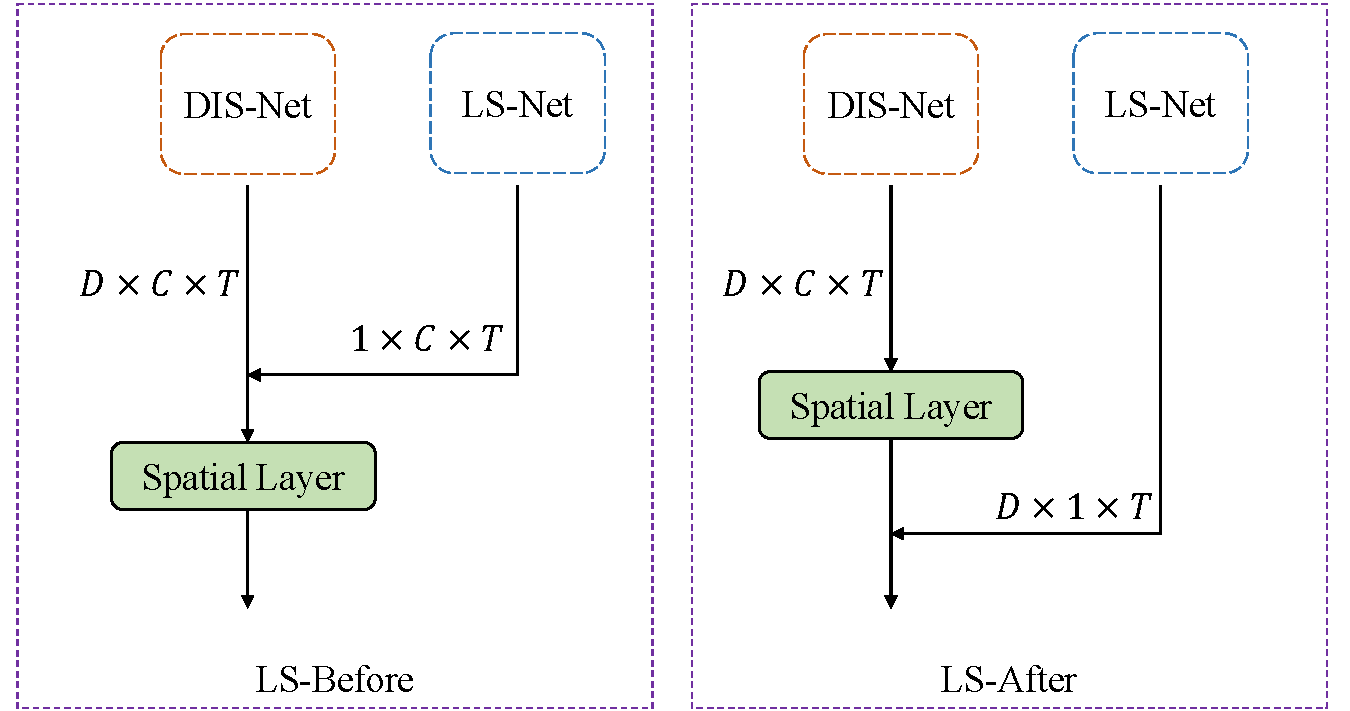
\includegraphics[width=0.6\textwidth]{fuse.pdf}
    \caption{不同融合方式}
    \label{fig:fuse}
\end{figure}

论文在2A数据集上使用HA-FuseNet进行实验,对这两种方式的效果予以验证。实验中对相关超参数进行了固定,从而只关注不同融合方式对性能造成的影响,表~\ref{tab:fuse}~对实验数据进行了展示,其中,准确率与Kappa系数为九位被试的平均表现。
\begin{table}[ht]
    \centering
    \caption{轻量化卷积模块实验结果对比}
    \label{tab:fuse}
    \begin{tabularx}{\textwidth}{CCCC}
      \toprule
      Models & ACC(\%) & Kappa & SD \\
      \midrule
      LS-Before & \textbf{75.66} & \textbf{0.67} & \textbf{9.71} \\
      LS-After & 74.54 & 0.66 & 11.94 \\
      \bottomrule
    \end{tabularx}
\end{table}

数据显示,LS-Before具有更高的准确率和一致性,且不同被试的准确率差异较小,这可能是因为LS-Net主要进行了时序特征提取与全局时空自注意力加权两个操作,对空间维度的操作较缺乏,因此需要由空间卷积层进行空间维度的特征提取,以获得更丰富的特征表达。论文采用LS-Before的方式进行LS-Net和DIS-Net的特征融合。

\subsection{各模块消融实验}

为了探究论文所提出的各个模块的有效性,并研究不同模块对HA-FuseNet分类效果的影响,论文针对这些模块进行消融实验,即按照模型构建的顺序,从基准模型开始,逐步对新增模块后的模型效果进行实验验证。

论文对不同结构的模型作以下定义:

(1) Inception:针对EEG信号的特点,修改了卷积核的基础Inception模型,具有三个Inception模块;

(2) Base-Inception:Inception+Bottleneck,即论文所提出的BaseNet。在inception模型的基础上引入反转瓶颈层,并对分支数量、激活函数等进行了调整;

(3) BI+Dense:Inception+Bottleneck+Dense Block,即论文所提出的DI-Net。在BaseNet的基础上,引入了密集连接模块;

(4) DI+svSE:Inception+Bottleneck+Dense Block+svSE,即论文所提出的DIS-Net。在DI-Net的基础上,引入了svSE混合注意力模块;

(5) DIS+LSTM:Inception+Bottleneck+Dense Block+svSE+LSTM。在DIS-Net的基础上,引入了LSTM网络;

(6) DIS+LSTM+SCoT:Inception+Bottleneck+Dense Block+svSE+LSTM+SCoT,即论文所提出的结合了DIS-Net和LS-Net的HA-FuseNet。在DIS+LSTM的基础上,引入了SCoT全局自注意力模块。

论文在2A数据集上进行消融实验,实验结果如表~\ref{tab:ab}~所示,其中,准确率和Kappa系数是九位被试的平均结果。

\begin{table}[ht]
    \centering
    \caption{HA-FuseNet各模块消融实验结果对比}
    \label{tab:ab}
    \begin{tabularx}{\textwidth}{CCCC}
      \toprule
      Models & ACC(\%) & Kappa & SD \\
      \midrule
      Inception \\
      Base-Inception \\
      BI+Dense \\
      DI+svSE \\
      DIS+LSTM \\
      DIS+LSTM+SCoT \\
      \bottomrule
    \end{tabularx}
\end{table}

实验数据显示,Inception+Bottleneck+Dense Block+svSE+LSTM+SCoT结构,即本文所提出的最终模型HA-FuseNet在MI-EEG分类任务上表现最好,准确率、Kappa一致性系数分别达到了,标准差达到了,证明在不同被试上,HA-FuseNet取得了最好的分类性能,且被试之间的准确率差异较小,具有较好的稳定性。此外,加入模块后模型的性能提升最大,

\subsection{BCI Competition IV Dataset 2A数据集上的对比试验}

在相同的实验设置下,论文在BCI Competition IV Dataset 2A数据集上进行HA-FuseNet与其他模型的被试内(Subject Dependent)对比试验和被试间(Subject Independent)对比实验,以对HA-FuseNet相对于其他模型在MI-EEG分类任务中的性能进行评估。

论文所使用的与HA-FuseNet进行对比的模型中,ShallowConvNet\cite{schirrmeister2017deep}与DeepConvNet\cite{schirrmeister2017deep}是基于卷积神经网络搭建;EEGNet\cite{lawhern2018eegnet}参考了BCI领域经典算法FBCSP的思想,将深度可分离卷积引入了网络结构中;EEGResNet\cite{HBM:HBM23730}基于残差神经网络\cite{he2016deep}构建;EEGInception\cite{zhang2021eeg}使用了Inception多分支和残差连接;EEGConformer\cite{song2022eeg}使用Transformer\cite{vaswani2017attention}与卷积神经网络串联,用以EEG信号的解码;LMDA-Net\cite{miao2023lmda}提出了一种新颖的通道注意力模块和深度注意力模块,基于ShallowConvNet和EEGNet进行了改进。

\paragraph{被试内对比试验}

2A数据集共有九名被试,每名被试具有独立的训练集和测试集,被试内对比实验即使用每名被试的训练集进行训练,在对应的测试集上进行测试,即为每名被试训练了一个模型。

表~\ref{tab:2acomparein}~展示了不同模型进行被试内实验的准确率,需要说明的是,在表~\ref{tab:2acomparein}~中未进行数据增强。表~\ref{tab:2acompareinsd}展示了被试内实验的Kappa一致性系数和标准差,其中,Kappa一致性系数为九名被试的平均值。

\begin{table}[ht]
    \centering
    \caption{HA-FuseNet与其他模型在测试集上的被试内实验结果对比(Acc)}
    \label{tab:2acomparein}
    \begin{subtable}[ht]{\textwidth}
      \centering
    %   \caption{子表a}
      \label{tab:2acompareina}
      \begin{tabularx}{\textwidth}{CCCCCC}
        \toprule
        Models & 1 & 2 & 3 & 4 & 5\\
        \midrule
        ShallowConvNet\cite{schirrmeister2017deep} & 85.07 & 61.46 & 94.10 & 73.26 & 73.26 \\
        DeepConvNet\cite{schirrmeister2017deep} & 83.68 & 65.28 & 90.63 & 69.44 & 76.04 \\
        EEGNet\cite{lawhern2018eegnet} & 78.13 & 63.54 & 82.30 & 60.42 & 71.88 \\
        EEGResNet\cite{HBM:HBM23730} & 69.10 & 40.97 & 63.89 & 49.65 & 45.49 \\
        EEGInception\cite{zhang2021eeg} & 71.18 & 48.26 & 82.29 & 55.90 & 64.58 \\
        EEGConformer\cite{song2022eeg} & 67.71 & 55.21 & 84.72 & 53.82 & 75.69 \\
        LMDA-Net\cite{miao2023lmda} & 86.46 & 60.46 & 90.97 & 59.02 & 69.10 \\
        \midrule 
        HA-FuseNet  & 91.67 & 61.81 & 91.67 & 63.19 & 75.00\\
        HA-FuseNet(SG) & 86.81 & 63.89 & 92.01 & 63.54 & 71.88\\
        \bottomrule
      \end{tabularx}
    \end{subtable}
    \begin{subtable}[ht]{\textwidth}
      \centering
    %   \caption{子表b}
      \label{tab:2acompareinb}
      \begin{tabularx}{\textwidth}{CCCCCCC}
        \toprule
        Models & 6 & 7 & 8 & 9 & Average \\
        \midrule
        ShallowConvNet\cite{schirrmeister2017deep} & 57.29 & 86.81 & 89.93 & 85.42 & 78.51\\
        DeepConvNet\cite{schirrmeister2017deep} & 64.58 & 89.93 & 79.51 & 73.61 & 76.97 \\
        EEGNet\cite{lawhern2018eegnet} & 59.03 & 72.92 & 68.06 & 66.67 & 69.21 \\
        EEGResNet\cite{HBM:HBM23730} & 42.36 & 54.51 & 61.11 & 64.93 & 54.67 \\
        EEGInception\cite{zhang2021eeg} & 52.43 & 75.00 & 85.41 & 73.61 & 67.63 \\
        EEGConformer\cite{song2022eeg} & 53.47 & 69.10 & 71.53 & 58.68 & 65.55 \\
        LMDA-Net\cite{miao2023lmda} & 55.90 & 90.28 & 81.94 & 76.04 & 74.50 \\
        \midrule 
        HA-FuseNet  & 65.97 & 89.58 & 81.60 & 78.47 & 77.66 \\
        HA-FuseNet(SG)  & 62.85 & 91.67 & 83.68 & 74.65 & 76.77 \\
        \bottomrule
      \end{tabularx}
    \end{subtable}
    
\end{table}

\begin{table}[ht]
    \centering
    \caption{HA-FuseNet与其他模型在测试集上的被试内实验结果对比(Kappa/SD)}
    \label{tab:2acompareinsd}
    \begin{tabularx}{\textwidth}{CCC}
      \toprule
      Models & Kappa & SD \\
      \midrule
      ShallowConvNet\cite{schirrmeister2017deep} & 0.70 & 12.15\\
      DeepConvNet\cite{schirrmeister2017deep} & 0.69 & 9.22 \\
      EEGNet\cite{lawhern2018eegnet} & 0.60 & 7.40 \\
      EEGResNet\cite{HBM:HBM23730} & 0.36 & 9.94 \\
      EEGInception\cite{zhang2021eeg} & 0.56 & 12.41 \\
      EEGConformer\cite{song2022eeg} & 0.53 & 10.33 \\
      LMDA-Net\cite{miao2023lmda} & 0.65 & 13.01 \\
      \midrule 
      HA-FuseNet &0.70&11.33\\
      HA-FuseNet(SG) &0.69&11.38\\
      \bottomrule
    \end{tabularx}
\end{table}

实验结果显示,

表~\ref{tab:2acompareag}~展示了进行数据增强后各模型在2A数据集上的被试内实验结果。

\begin{table}[ht]
    \centering
    \caption{数据增强后HA-FuseNet与其他模型在测试集上的被试内实验结果对比(Acc)}
    \label{tab:2acompareag}
    \begin{subtable}[ht]{\textwidth}
      \centering
    %   \caption{子表a}
      \label{tab:2acompareaga}
      \begin{tabularx}{\textwidth}{CCCCCC}
        \toprule
        Models & 1 & 2 & 3 & 4 & 5\\
        \midrule
        ShallowConvNet\cite{schirrmeister2017deep}  & 89.72 & 66.20 & 94.34 & 84.54 & 76.39 \\
        DeepConvNet\cite{schirrmeister2017deep} & 82.58 & 62.37 & 91.11 & 73.14 & 69.18 \\
        EEGNet\cite{lawhern2018eegnet} & 77.61 & 67.77 & 94.95 & 66.25 & 61.63 \\
        EEGResNet\cite{HBM:HBM23730} & 77.88 & 53.05 & 76.22 & 65.37 & 49.39 \\
        EEGInception\cite{zhang2021eeg}  & 88.07 & 61.93 & 91.29 & 77.83 & 69.97 \\
        EEGConformer\cite{song2022eeg}  & 80.05 & 47.82 & 85.98 & 25.27 & 58.25 \\
        LMDA-Net\cite{miao2023lmda} & 88.15 & 69.16 & 91.99 & 81.18 & 70.31 \\
        \midrule 
        HA-FuseNet \\
        \bottomrule
      \end{tabularx}
    \end{subtable}
    \begin{subtable}[ht]{\textwidth}
      \centering
    %   \caption{子表b}
      \label{tab:2acompareagb}
      \begin{tabularx}{\textwidth}{CCCCCCC}
        \toprule
        Models & 6 & 7 & 8 & 9 & Average \\
        \midrule
        ShallowConvNet\cite{schirrmeister2017deep}  & 62.24 & 96.69 & 90.94 & 89.55 & 83.40 \\
        DeepConvNet\cite{schirrmeister2017deep}  & 59.38 & 86.85 & 85.80 & 82.58 & 77.00 \\
        EEGNet\cite{lawhern2018eegnet} & 46.09 & 85.80 & 83.71 & 87.63 & 74.61 \\
        EEGResNet\cite{HBM:HBM23730}  & 44.44 & 77.61 & 75.35 & 61.85 & 64.57 \\
        EEGInception\cite{zhang2021eeg} & 57.03 & 90.33 & 84.76 & 84.58 & 78.42 \\
        EEGConformer\cite{song2022eeg}  & 26.65 & 52.27 & 27.00 & 25.61 & 47.65 \\
        LMDA-Net\cite{miao2023lmda}& 60.24 & 93.21 & 83.28 & 86.41 & 80.44 \\
        \midrule 
        HA-FuseNet \\
        \bottomrule
      \end{tabularx}
    \end{subtable}
    
\end{table}

\begin{table}[ht]
    \centering
    \caption{数据增强后HA-FuseNet与其他模型在测试集上的被试间实验结果对比(Kappa/SD)}
    \label{tab:2acompareagsd}
    \begin{tabularx}{\textwidth}{CCC}
      \toprule
      Models & Kappa & SD \\
      \midrule
      ShallowConvNet\cite{schirrmeister2017deep} & 0.78 & 11.67 \\
      DeepConvNet\cite{schirrmeister2017deep} & 0.69 & 10.73 \\
      EEGNet\cite{lawhern2018eegnet} & 0.66 & 14.52 \\
      EEGResNet\cite{HBM:HBM23730} & 0.53 & 12.36 \\
      EEGInception\cite{zhang2021eeg} & 0.71 & 11.92 \\
      EEGConformer\cite{song2022eeg} & 0.30 & 22.38 \\
      LMDA-Net\cite{miao2023lmda} & 0.74 & 10.74 \\
      \midrule 
      HA-FuseNet \\
      \bottomrule
    \end{tabularx}
\end{table}

\paragraph{被试间对比试验}

在被试间对比实验中,对于被试\(i\),使用全部其他被试的训练集为被试\(i\)的训练集,如公式~\ref{eq:cross}~所示,其中,\(Train_j\)表示被试\(j\)的训练集。仍然使用被试\(i\)的测试集为测试集。
\begin{equation}
    \label{eq:cross}
    Train_i=\sum_{j}^{N}Train_j,\,i \in [1,9],\,j \in [1,9],\,j \neq i
\end{equation}

表~\ref{tab:2acomparecross}~展示了各个模型进行被试间实验的准确率结果对比,例如,表格中[ShallowConvNet,1]即表示ShallowConvNet使用其他八名被试的训练集集合,在1号被试的测试集上得到的准确率。表~\ref{tab:2acomparecrosssd}~展示了被试间实验的Kappa系数和标准差结果对比,其中,Kappa系数为九名被试的平均值。被试间对比试验没有使用数据增强算法。

\begin{table}[ht]
    \centering
    \caption{HA-FuseNet与其他模型在测试集上的被试间实验结果对比(Acc)}
    \label{tab:2acomparecross}
    \begin{subtable}[ht]{\textwidth}
      \centering
    %   \caption{子表a}
      \label{tab:2acomparecrossa}
      \begin{tabularx}{\textwidth}{CCCCCC}
        \toprule
        Models & 1 & 2 & 3 & 4 & 5\\
        \midrule
        ShallowConvNet\cite{schirrmeister2017deep}   & 76.39 & 52.78 & 71.53 & 26.04 & 50.69\\
        DeepConvNet\cite{schirrmeister2017deep} & 71.53 & 50.69 & 84.72 & 61.46 & 69.10 \\
        EEGNet\cite{lawhern2018eegnet} & 68.75 & 56.60 & 68.75 & 61.11 & 68.75 \\
        EEGResNet\cite{HBM:HBM23730} & 61.81 & 38.54 & 64.24 & 45.83 & 39.93 \\
        EEGInception\cite{zhang2021eeg}  & 74.31 & 51.04 & 81.60 & 52.43 & 56.25 \\
        EEGConformer\cite{song2022eeg}  & 52.78 & 26.04 & 26.04 & 50.00 & 64.24\\
        LMDA-Net\cite{miao2023lmda} & 72.22 & 47.22 & 83.68 & 55.90 & 51.74 \\
        \midrule 
        HA-FuseNet  & 76.04 & 44.79 & 84.72 & 55.21 & 53.12\\
        \bottomrule
      \end{tabularx}
    \end{subtable}
    \begin{subtable}[ht]{\textwidth}
      \centering
    %   \caption{子表b}
      \label{tab:2acomparecrossb}
      \begin{tabularx}{\textwidth}{CCCCCCC}
        \toprule
        Models & 6 & 7 & 8 & 9 & Average \\
        \midrule
        ShallowConvNet\cite{schirrmeister2017deep}  & 74.31 & 27.78 & 64.93 & 72.92 & 57.38\\
        DeepConvNet\cite{schirrmeister2017deep} & 59.03 & 75.35 & 74.31 & 64.93 & 67.9 \\
        EEGNet\cite{lawhern2018eegnet}  & 58.68 & 73.61 & 56.60 & 56.25 & 63.23 \\
        EEGResNet\cite{HBM:HBM23730}  & 42.01 & 47.22 & 50.69 & 56.25 & 49.61 \\
        EEGInception\cite{zhang2021eeg}  & 60.42 & 71.18 & 73.96 & 74.31 & 66.17 \\
        EEGConformer\cite{song2022eeg} & 25.00 & 26.74 & 29.51 & 27.78 & 36.46\\
        LMDA-Net\cite{miao2023lmda}  & 48.26 & 71.88 & 76.04 & 66.67 & 63.73\\
        \midrule 
        HA-FuseNet  & 50.35 & 76.74 & 77.08 & 68.06 & 65.12 \\
        \bottomrule
      \end{tabularx}
    \end{subtable}
    
\end{table}

\begin{table}[ht]
    \centering
    \caption{HA-FuseNet与其他模型在测试集上的被试间实验结果对比(Kappa/SD)}
    \label{tab:2acomparecrosssd}
    \begin{tabularx}{\textwidth}{CCC}
      \toprule
      Models & Kappa & SD \\
      \midrule
      ShallowConvNet\cite{schirrmeister2017deep} &0.43&19.32 \\
      DeepConvNet\cite{schirrmeister2017deep} &0.57&9.54\\
      EEGNet\cite{lawhern2018eegnet} &0.51& 6.33\\
      EEGResNet\cite{HBM:HBM23730} &0.33&8.83\\
      EEGInception\cite{zhang2021eeg} &0.55&10.57\\
      EEGConformer\cite{song2022eeg}&0.15&14.09 \\
      LMDA-Net\cite{miao2023lmda} &0.52&12.53\\
      \midrule 
      HA-FuseNet &0.53&13.6\\
      \bottomrule
    \end{tabularx}
\end{table}


\subsection{BCI Competition IV Dataset 2B数据集上的对比试验}

\begin{table}[ht]
    \centering
    \caption{HA-FuseNet与其他模型在测试集上的被试内实验结果对比(Acc)}
    
    \begin{subtable}[ht]{\textwidth}
      \centering
    %   \caption{子表a}
      \label{tab:2bcompareina}
      \begin{tabularx}{\textwidth}{CCCCCC}
        \toprule
        Models & 1 & 2 & 3 & 4 & 5\\
        \midrule
        ShallowConvNet\cite{schirrmeister2017deep} & 59.17 & 68.33 & 74.17 & 60.83 & 63.08\\
        DeepConvNet\cite{schirrmeister2017deep} & 59.17 & 76.67 & 72.50 & 60.00 & 68.46\\
        EEGNet\cite{lawhern2018eegnet} & 60.00 & 72.50 & 73.33 & 57.50 & 59.23 \\
        EEGResNet\cite{HBM:HBM23730} \\
        EEGInception\cite{zhang2021eeg} \\
        EEGConformer\cite{song2022eeg} \\
        LMDA-Net\cite{miao2023lmda} \\
        \midrule 
        HA-FuseNet \\
        \bottomrule
      \end{tabularx}
    \end{subtable}
    \begin{subtable}[ht]{\textwidth}
      \centering
    %   \caption{子表b}
      \label{tab:2bcompareinb}
      \begin{tabularx}{\textwidth}{CCCCCCC}
        \toprule
        Models & 6 & 7 & 8 & 9 & Average \\
        \midrule
        ShallowConvNet\cite{schirrmeister2017deep} & 80.83 & 59.29 & 90.77 & 78.33 & 70.53 \\
        DeepConvNet\cite{schirrmeister2017deep} & 80.00 & 63.57 & 97.69 & 78.33 & 72.93 \\
        EEGNet\cite{lawhern2018eegnet} & 66.67 & 57.86 & 94.62 & 78.33 & 68.89 \\
        EEGResNet\cite{HBM:HBM23730} \\
        EEGInception\cite{zhang2021eeg} \\
        EEGConformer\cite{song2022eeg} \\
        LMDA-Net\cite{miao2023lmda} \\
        \midrule 
        HA-FuseNet \\
        \bottomrule
      \end{tabularx}
    \end{subtable}
    
\end{table}

\begin{table}[ht]
    \centering
    \caption{HA-FuseNet与其他模型在测试集上的被试内实验结果对比(Kappa/SD)}
    \label{tab:2bcompareinsd}
    \begin{tabularx}{\textwidth}{CCC}
      \toprule
      Models & Kappa & SD \\
      \midrule
      ShallowConvNet\cite{schirrmeister2017deep} &&10.54\\
      DeepConvNet\cite{schirrmeister2017deep} &&11.40\\
      EEGNet\cite{lawhern2018eegnet} && 11.61\\
      EEGResNet\cite{HBM:HBM23730} &&\\
      EEGInception\cite{zhang2021eeg} &&\\
      EEGConformer\cite{song2022eeg} &&\\
      LMDA-Net\cite{miao2023lmda} &&\\
      \midrule 
      HA-FuseNet \\
      \bottomrule
    \end{tabularx}
\end{table}



\begin{table}[ht]
    \centering
    \caption{HA-FuseNet与其他模型在测试集上的被试间实验结果对比(Acc)}
    
    \begin{subtable}[ht]{\textwidth}
      \centering
    %   \caption{子表a}
      \label{tab:2bcomparecrossa}
      \begin{tabularx}{\textwidth}{CCCCCC}
        \toprule
        Models & 1 & 2 & 3 & 4 & 5\\
        \midrule
        ShallowConvNet\cite{schirrmeister2017deep} \\
        DeepConvNet\cite{schirrmeister2017deep} \\
        EEGNet\cite{lawhern2018eegnet} \\
        EEGResNet\cite{HBM:HBM23730} \\
        EEGInception\cite{zhang2021eeg} \\
        EEGConformer\cite{song2022eeg} \\
        LMDA-Net\cite{miao2023lmda} \\
        \midrule 
        HA-FuseNet \\
        \bottomrule
      \end{tabularx}
    \end{subtable}
    \begin{subtable}[ht]{\textwidth}
      \centering
    %   \caption{子表b}
      \label{tab:2bcomparecrossb}
      \begin{tabularx}{\textwidth}{CCCCCCC}
        \toprule
        Models & 6 & 7 & 8 & 9 & Average \\
        \midrule
        ShallowConvNet\cite{schirrmeister2017deep} \\
        DeepConvNet\cite{schirrmeister2017deep} \\
        EEGNet\cite{lawhern2018eegnet} \\
        EEGResNet\cite{HBM:HBM23730} \\
        EEGInception\cite{zhang2021eeg} \\
        EEGConformer\cite{song2022eeg} \\
        LMDA-Net\cite{miao2023lmda} \\
        \midrule 
        HA-FuseNet \\
        \bottomrule
      \end{tabularx}
    \end{subtable}
    
\end{table}

\begin{table}[ht]
    \centering
    \caption{HA-FuseNet与其他模型在测试集上的被试间实验结果对比(Kappa/SD)}
    \label{tab:2bcomparecrosssd}
    \begin{tabularx}{\textwidth}{CCC}
      \toprule
      Models & Kappa & SD \\
      \midrule
      ShallowConvNet\cite{schirrmeister2017deep} \\
      DeepConvNet\cite{schirrmeister2017deep} \\
      EEGNet\cite{lawhern2018eegnet} \\
      EEGResNet\cite{HBM:HBM23730} \\
      EEGInception\cite{zhang2021eeg} \\
      EEGConformer\cite{song2022eeg} \\
      LMDA-Net\cite{miao2023lmda} \\
      \midrule 
      HA-FuseNet \\
      \bottomrule
    \end{tabularx}
\end{table}

\section{本章小结}

